\documentclass{article}
\usepackage[utf8]{inputenc}
\usepackage[none]{hyphenat}
\usepackage[a4paper, total={7in, 9in}]{geometry}
\usepackage{fancyhdr}
\usepackage{parskip}
\usepackage{hyperref}
\usepackage{booktabs}
\usepackage{graphicx}
\usepackage{subcaption}

\title{Classification of Music Genres of Billboard Hot Songs with Spotify}
\author{Yuwei (Johnny) Meng}
\date{30 Apr 2024}

\begin{document}

\pagestyle{fancy}
\fancyhead[L]{30 Apr 2024}
\fancyhead[C]{Music Genre Classification}
\fancyhead[R]{Johnny Meng}

\maketitle

\href{https://github.com/BullDF/billboard-songs-analysis-with-spotify/tree/main}{\textbf{Source Code on GitHub}}

\href{https://bulldf.github.io/billboard-songs-analysis-with-spotify/}{\textbf{Project Website}}

\href{https://play.library.utoronto.ca/watch/c4d71902f00f5e6fe91bea00974fce6c}{\textbf{Project Presentation}}

\section{Introduction}

Music, as a human culture, takes a large part in people's life for long. In the current era where technology thrives, countless digital musical softwares emerge, granting listeners with access to music at anytime, anywhere in the world. Concurrently emerged is the booming development of various music genres, each with its unique musical characteristics. Therefore, classifying music genres is an interesting research topic because, for one reason, a successful classification model can give insight into building a song recommendation system.

As an entry point to the project, a dataset on the ``Hot 100'' Billboard songs every week starting from 1958 is downloaded from Kaggle. The dataset contains 330087 rows and 7 columns that include information about the date of the song on Billboard, the name, the artist(s), and the rank on Billboard. In this project, only the name and the artist(s) columns are used.

Among the leading musical softwares, Spotify is a world-changing one. Founded in 2006 in Sweden, Spotify gradually attracted more and more users and built up a massive repository of worldwide music. Of this reason, a major portion of the data utilized in this data analysis project is obtained from Spotify through the Spotify web API and deemed credible and reliable. This portion of data contains the name of tracks, the artist(s), the track popularity, some audio features (see \hyperref[sec:audio_features]{appendix A} for full list) and in particular, a genre of music that the artist performs.

This project aims to use the aforementioned information extracted from Spotify to build and compare multiple machine learning models for the sake of classifying music genres. The models are evaluated through classification accuracy score.

\section{Methodology}

The Billboard hot songs dataset from Kaggle is used as a reference. Starting with this list of 330087 tracks, to prevent overloading the Spotify API and keep the data at a manageable size, I randomly sampled 5000 tracks for the remaining analysis. Then I used the Spotify web API via the \texttt{Spotipy} Python library to access these songs on Spotify and extracted the audio features and popularity for these 5000 tracks. Given that some of these tracks are unavailable on Spotify, I eventually obtained a dataset of 3823 tracks with their corresponding audio features. To get the labels, I selected 7 famous music genres (see \hyperref[sec:select_music_genres]{appendix B}). The Spotify API was then used to extract the music genre that the artists perform. If the music genre for an artist is not on the list, then the artist was marked as \textit{other}. For analysis, I merged the information into a single dataset with all the audio features and the genres of the tracks and split the dataset into a training set and a test set using an 80:20 ratio. All data wrangling steps were completed in R.

For the classification task, I constructed multiple machine learning models on the training set and evaluated them on the test set. These models included decision tree, random forest, gradient boosting, extreme gradient boosting (XGBoost), Gaussian Naive Bayes (GaussianNB), and neural network. The model construction and evaluation process was completed entirely in Python. The decision tree, random forest, gradient boosting, and GaussianNB models were constructed using the \texttt{scikit-learn} package. For some models, I ran a \(k\)-fold cross-validation to search over a set of hyperparameters (see \hyperref[sec:hyperparameters]{appendix C}). The XGBoost model was built using the \texttt{XGBoost} package. For comparison, I constructed two XGBoost models with different hyperparameters. The neural network featured 3 fully-connected layers and an output layer, implemented using the \texttt{PyTorch} framework. Batch normalization and dropout layers were included. The ReLU function was applied as activation throughout the model and the cross-entropy loss was used for the optimization task. Upon construction, all models were evaluated on the test dataset using accuracy score.

\section{Exploratory Data Analysis}

Most exploratory data analysis steps have been completed in a previous part of this project (see EDA \href{https://github.com/BullDF/billboard-songs-analysis-with-spotify/blob/main/EDA/report.pdf}{report} and \href{https://bulldf.github.io/billboard-songs-analysis-with-spotify/EDA.html}{interactive visualizations}). Here I present some additional exploratory data analysis pertaining to the music genres for the following machine learning analysis.

\autoref*{fig:music_genres} below shows the counts of music genres in the entire dataset:

\begin{figure}[htbp]
    \centering
    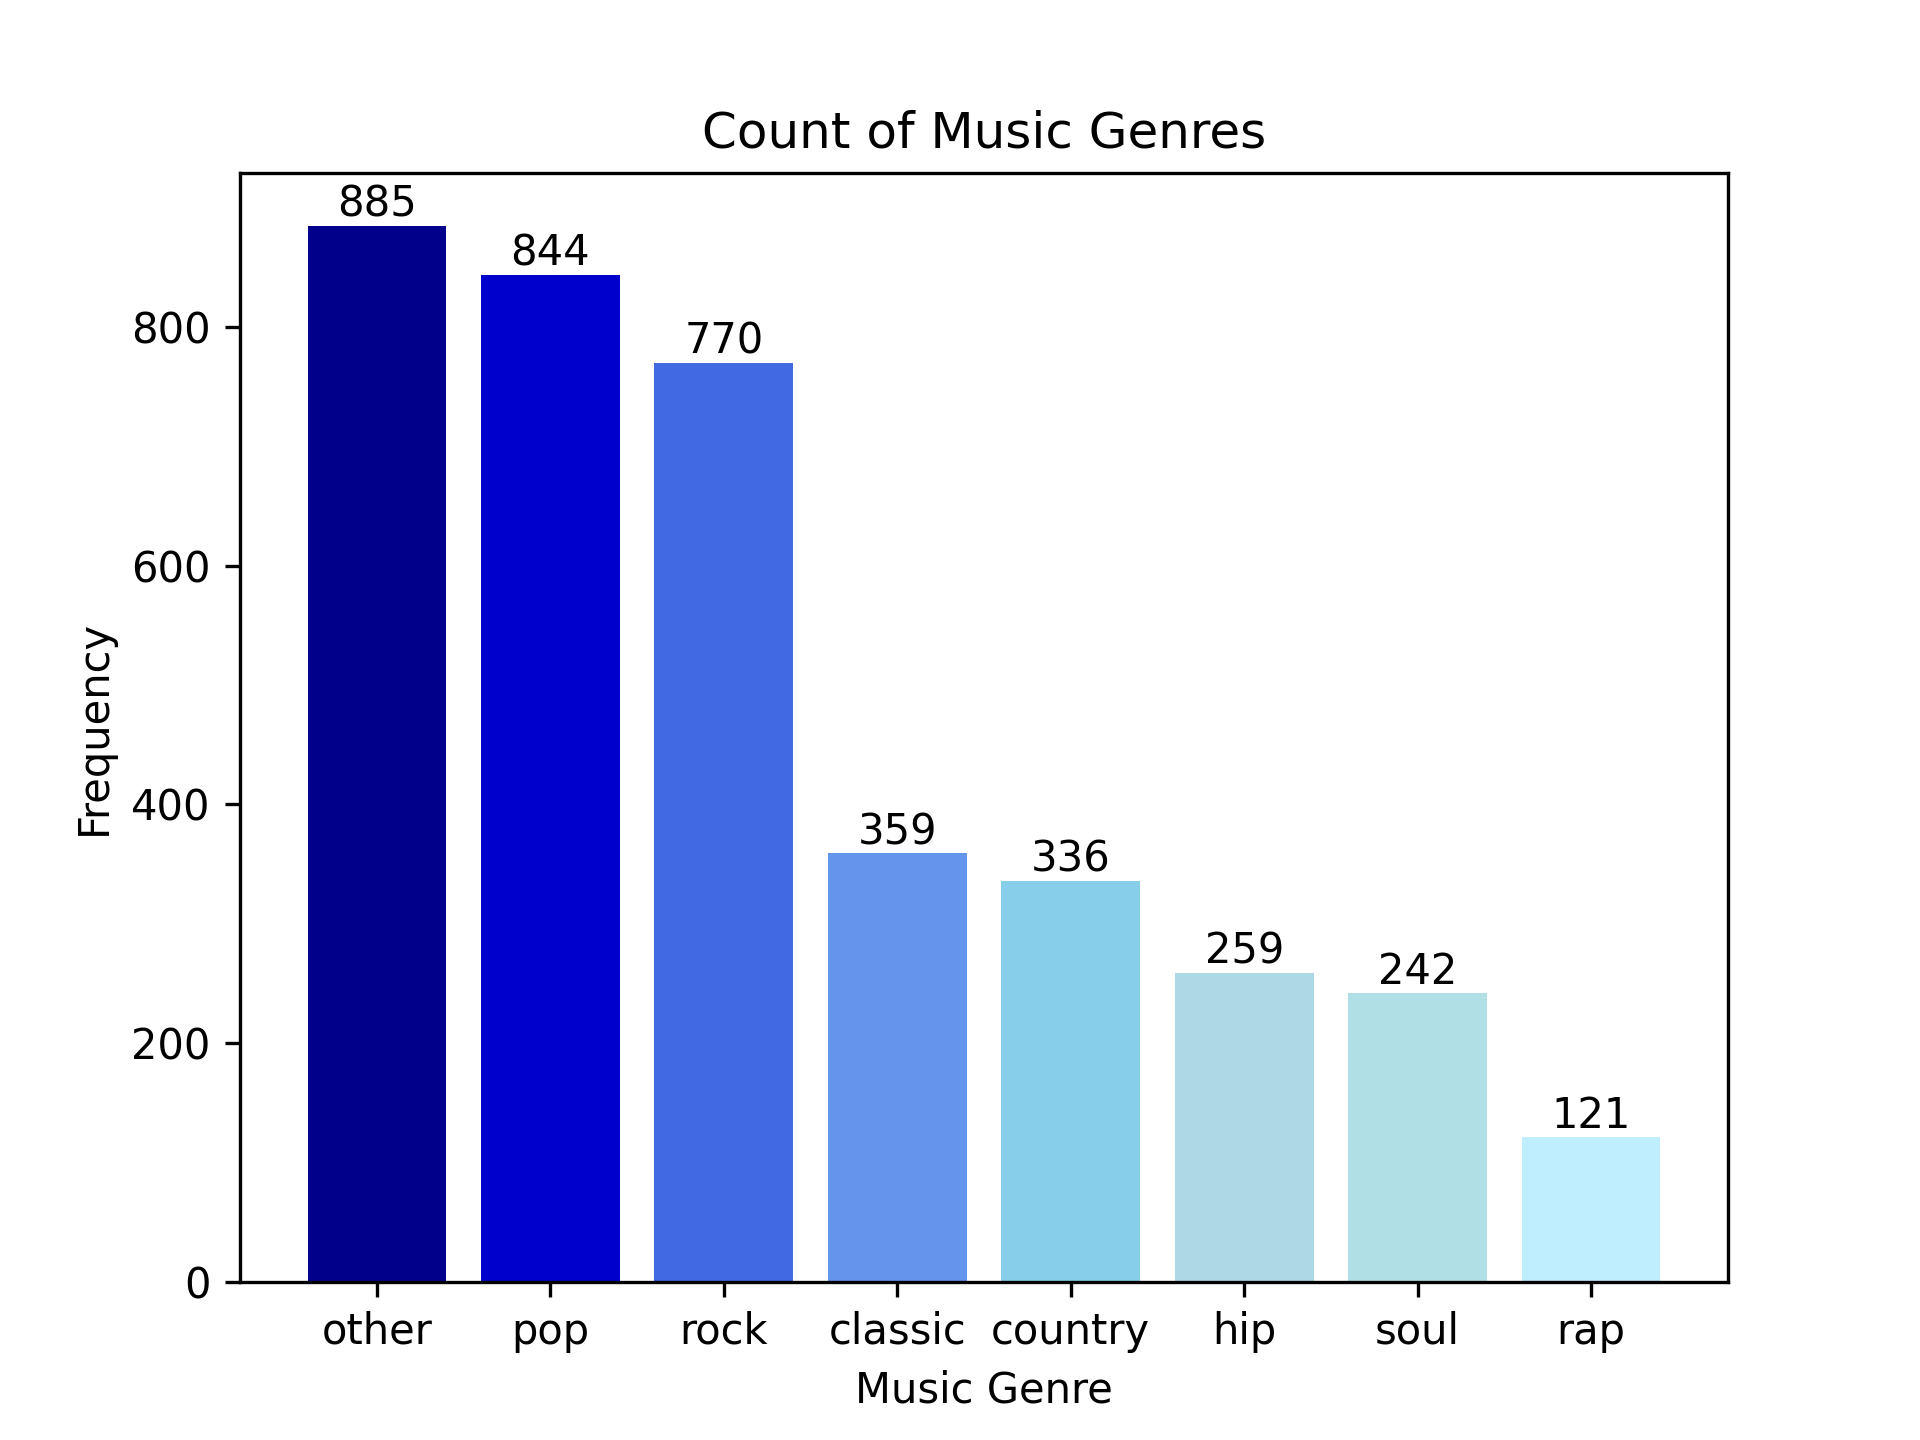
\includegraphics[width=15cm]{count_of_music_genres.png}
    \caption{Count of Music Genres}
    \label{fig:music_genres}
\end{figure}

From the plot, we can see that the number of tracks in each music genre is very unbalanced, with the \textit{other} genre having the highest number of 885 and \textit{rap} having the lowest number of 121. This poses a potential problem in the subsequent classification task as most models perform poorly on unbalanced data due to inability to learn the structure behind the data entirely.

\section{Results}

\autoref*{tab:model_performance} shows the training accuracy and test accuracy for each built machine learning model in the analysis. Models suffixed as \textit{Default} were fitted using the default hyperparameters defined in \texttt{scikit-learn} and models suffixed as \textit{CV} were fitted through \(k\)-fold cross-validation.

\begin{table}[htbp]
    \centering
    \begin{tabular}{lcc}
        \toprule
        \textbf{Model} & \textbf{Training Accuracy} & \textbf{Test Accuracy} \\
        \midrule
        Decision Tree Default & 0.971 & 0.356 \\[3pt]
        Decision Tree CV & 0.487 & 0.440 \\[3pt]
        \textbf{Random Forest Default} & \textbf{0.971} & \textbf{0.505} \\[3pt]
        Random Forest CV & 0.804 & 0.473 \\[3pt]
        Gradient Boosting Default & 0.739 & 0.488 \\[3pt]
        Gradient Boosting CV & 0.509 & 0.436 \\[3pt]
        XGBoost with \(\eta = 0.1\) & 0.750 & 0.482 \\[3pt]
        XGBoost with \(\eta = 0.001\) & 0.596 & 0.443 \\[3pt]
        Gaussian Naive Bayes & 0.358 & 0.372 \\[3pt]
        Neural Network without Dropout & 0.861 & 0.442 \\[3pt]
        Neural Network with Dropout & 0.551 & 0.486 \\
        \bottomrule
    \end{tabular}
    \caption{Model Performance}
    \label{tab:model_performance}
\end{table}

From \autoref*{tab:model_performance}, we notice that the default random forest achieved the highest test accuracy of 0.505. The CV random forest, the default gradient boosting, the XGBoost model with \(\eta=0.1\), and the neural network also achieved comparable test accuracy. In contrast, the default decision tree and the Gaussian Naive Bayes had the lowest test accuracy.

We can use the default random forest and plot its feature importance. For comparison, the feature importance plot for the default decision tree is also plotted.

\begin{figure}[htbp]
    \centering
    \begin{subfigure}[b]{0.45\textwidth}
        \centering
        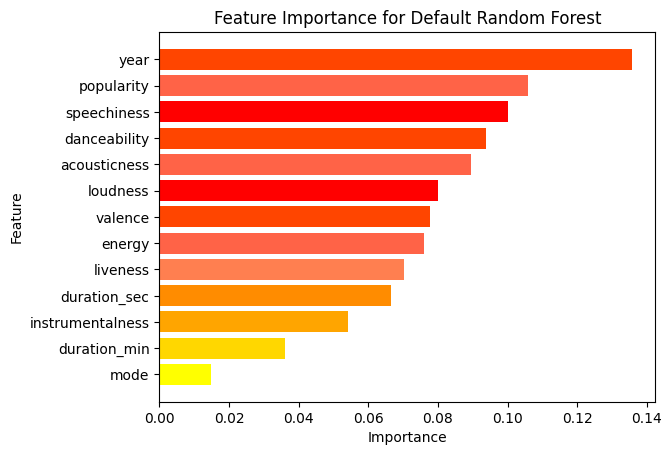
\includegraphics[width=\textwidth]{rf_var_imp.png}
        \caption{Default Random Forest}
    \end{subfigure}
    \hfill
    \begin{subfigure}[b]{0.45\textwidth}
        \centering
        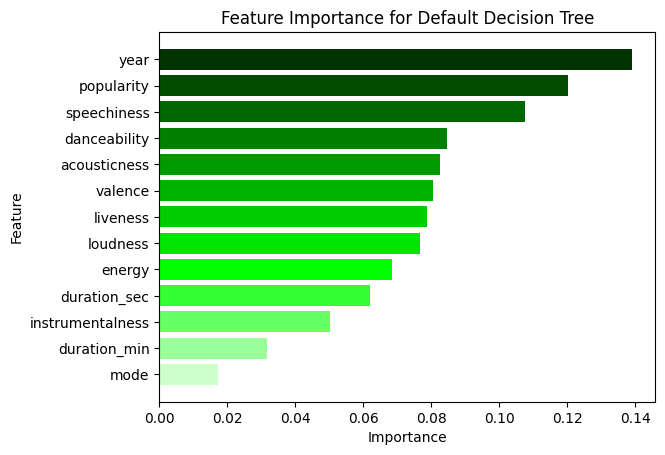
\includegraphics[width=\textwidth]{dt_var_imp.png}
        \caption{Default Decision Tree}
    \end{subfigure}
    \caption{Feature Importance}
    \label{fig:var_imp}
\end{figure}

From \autoref*{fig:var_imp}, we observe that the default random forest and the default decision tree agreed that \textit{year}, \textit{popularity}, \textit{speechiness}, \textit{danceability}, and \textit{acousticness} were the 5 most important features in the dataset in classifying the music genres. Additionally, \textit{mode}, \textit{duration}, and \textit{instrumentalness} were the least important features. This result might not be a coincidence and is explored further in the following section.

\section{Discussion}

The previous section provided an overview of the machine learning models trained for classifying music genres. This section explores the advantages and drawbacks of these models individually.

\subsection{Decision Tree}

From \autoref{tab:model_performance}, we noticed that the training accuracy for the default decision tree was very high, but the test accuracy was the poorest among all the models. This was not surprising since decision tree is notorious in overfitting and not robust to small variations in the data. With cross-validation, the training accuracy dropped down to 0.487, which did help in reducing overfitting, but the test accuracy didn't increase too much. Overall, decision tree is undoubtedly a simple model with only few assumptions and hence it is normal that decision tree did not perform too well, even with cross-validation.

\subsection{Random Forest}

Among all the trained models, the default random forest achieved the highest test accuracy of 0.505, predicting half of the test data correctly. The CV random forest also performed well. As an improvement to decision tree, random forest makes an ensemble of trees and averages the prediction output to reduce variance, which mitigates overfitting to the training data.

Something surprising to note is that the CV random forest was worse than the default random forest, since we expected cross-validation finds the best hyperparameters while reducing overfitting. Nevertheless, from the results we observe that both the default and the CV random forests were overfitting to the training data to a large extent since the training accuracy and the test counterpart greatly differed. Hence it is not unreasonable to attribute the high test accuracy for the default random forest to the randomness within the model architecture. Furthermore, in the default random forest, the \texttt{max\_depth} parameter was not set so that the model tried to fit the data until there was impunity. On the contrary, I specified a range of maximum depth values for cross-validation to search over in the CV random forest. Hence it is possible that the \texttt{max\_depth} values I set were not enough for the model to achieve great performance.

\subsection{Gradient Boosting}

Gradient boosting uses the boosting ensemble method. As opposed to random forest, which uses bagging to build multiple trees and outputs the averaged results, gradient boosting trains another model on the data that the previous model predicted wrong, so that the ensemble can capture nuances in the training data. From \autoref{tab:model_performance}, overfitting seems to be an issue for the default gradient boosting, since the training accuracy was a lot higher than the test accuracy, but the CV gradient boosting improved on this. Nevertheless, the CV gradient boosting also decreased in test accuracy. The supposed explanation will be presented in the following XGBoost section.

\subsection{XGBoost}

XGBoost is basically a gradient boosting model but with more regularization terms to reduce overfitting. However, overfitting was still a problem in the XGBoost model with a learning rate of \(\eta=0.1\). For the XGBoost with \(\eta=0.001\), overfitting was reduced but the accuracy decreased as well. From this analysis and the previous gradient boosting section, we can summarize that in the current classification task, we should favor large learning rates over small ones since the XGBoost with a larger learning rate outperformed its counterpart on both the training and test sets. For gradient boosting, the set of learning rates that I experimented with in the cross-validation was also smaller than the default learning rate, leading to poor performance even with cross-validation.

\subsection{Gaussian Naive Bayes}

The Gaussian NB model was actually the model that I expected to have the best performance among all. Being a probabilistic model, Gaussian NB assumes the input features are conditionally independent Gaussian random variables given the class labels. With a prior distribution, Gaussian NB computes the likelihood of an input vector in each of the classes and chooses the maximum as the prediction via Bayes' Rule. Considering the prior belief that each music genre has its unique characteristics, a probabilistic model should be capable of capturing the underlying pattern in the audio features of tracks.

One caveat that explains the poor performance of the Gaussian NB model is that, as we have seen in the \href{https://bulldf.github.io/billboard-songs-analysis-with-spotify/EDA.html}{EDA}, not all input features strictly follow a Gaussian distribution. For instance, the \textit{year} column is uniformly distributed and the \textit{speechiness} audio feature (and some others) is strongly skewed. The \textit{mode} attribute also follows a Bernoulli distribution, failing to satisfy the assumptions for Gaussian NB. To ameliorate the assumptions, a log transformation is helpful in turning the skewed audio features into a Gaussian distribution.

\subsection{Neural Network}

Similar to Gaussian NB, before model fitting I hypothesized that neural network would outperform other models in the classification of music genres. Through several hidden layers, neural network can learn complex, non-linear patterns behind the data. In this project, I experimented with two neural networks with the same architecture, but one with dropout in every layer and one without. From \autoref{tab:model_performance}, we noticed that the NN without dropout was overfitting to the training set, while the NN with dropout was more generalizable to the test set, which was expected. The test accuracy for both NNs was not high though. More experiments with the architecture and hyperparameter choices can be explored to build a better neural network in the future.

\subsection{Feature Importance}

To close this section, the feature importance plots in \autoref{fig:var_imp} deserves some discussion. Particularly, the \textit{year} that the track was on Billboard was the most important feature in determining the music genre. I suppose the reason is people's like changed over time and so each time period was associated with a certain hot music genre, thus making year a valuable determinant. \textit{Popularity} is a similar metric since it was defined to be related to time (for this reason, some multicollinearity was introduced in the dataset and it might lead to the poor performance of some models). The \textit{duration} and \textit{mode} features took the least important slots because \textit{duration} does not explicitly imply music genres and there were only 2 modes -- \textit{major} and \textit{minor} -- which was clearly not too informative given 8 music genres.

\section{Conclusion}

Through the above analysis, I constructed various machine learning models, including decision tree, bagging and boosting ensembles, Gaussian Naive Bayes as a probabilistic model, and neural network, for classifying music genres of Billboard hot songs. Among all the models, the random forest trained with the default hyperparameters on \texttt{scikit-learn} achieved the highest training accuracy of 0.971 and the highest test accuracy of 0.505. Other models were at the comparable level but with slightly lower accuracy.

\subsection{Limitations}

There are some limitations in the above analysis. The most important one is the validity of the data, especially the labels. Since the Spotify API does not have genre information available for the tracks, the way I created the labels was to look up the genres for the artists of the tracks and build the labels from this information. Hence the analysis was based on the assumption that the tracks were strictly in the same genres as the artists, which was generally not true. If possible, future research should incorporate precise track genres into the classification task. Nonetheless, a best final test accuracy of 0.505 implies that there is indeed some associations between the audio features and the artist genres, which is not completely meaningless.

Another limitation is the computation bottleneck. If resource permits, future research should extract a larger dataset and obtain a validation set to systematically tune hyperparameters for all models. This way researchers can fully explore the potentials of all models and evaluate accordingly. Hopefully the classification labels will be more balanced as well.

\section{Acknowledgements}

I would like to express my sincere gratitude to \href{https://meredithfranklin.github.io/}{Dr. Meredith Franklin} in the Department of Statistical Sciences at the University of Toronto for her valuable suggestions and comments towards completing this project.

\section{References}

\begin{itemize}
    \item \href{https://www.kaggle.com/datasets/dhruvildave/billboard-the-hot-100-songs}{Billboard ``The Hot 100'' Songs}
    \item \href{https://developer.spotify.com/documentation/web-api}{Spotify Web API Documentation}
    \item \href{https://spotipy.readthedocs.io/en/2.22.1/}{Spotipy Python Library Documentation}
    \item Python Package Documentations:
    \begin{itemize}
        \item \href{https://pytorch.org/docs/stable/torch.html}{\texttt{PyTorch}}
        \item \href{https://scikit-learn.org/stable/index.html}{\texttt{scikit-learn}}
        \item \href{https://xgboost.readthedocs.io/en/stable/python/python_intro.html}{\texttt{XGBoost}}
    \end{itemize}
\end{itemize}

\pagebreak

\section{Appendices}

\subsection*{Appendix A: Full List of Spotify Audio Features}\label{sec:audio_features}

\begin{table}[htbp]
    \centering
    \begin{tabular}{l p{0.7\textwidth}}
        \toprule
        \textbf{Audio Feature} & \textbf{Description} \\
        \midrule

        acousticness & A confidence measure from 0.0 to 1.0 of whether the track is acoustic. 1.0 represents high confidence the track is acoustic. \\[3pt]

        danceability & Danceability describes how suitable a track is for dancing based on a combination of musical elements including tempo, rhythm stability, beat strength, and overall regularity. A value of 0.0 is least danceable and 1.0 is most danceable. \\[3pt]

        duration\_ms & The duration of the track in milliseconds. \\[3pt]

        energy & Energy is a measure from 0.0 to 1.0 and represents a perceptual measure of intensity and activity. Typically, energetic tracks feel fast, loud, and noisy. For example, death metal has high energy, while a Bach prelude scores low on the scale. Perceptual features contributing to this attribute include dynamic range, perceived loudness, timbre, onset rate, and general entropy. \\[3pt]

        instrumentalness & Predicts whether a track contains no vocals. ``Ooh'' and ``aah'' sounds are treated as instrumental in this context. Rap or spoken word tracks are clearly ``vocal''. The closer the instrumentalness value is to 1.0, the greater likelihood the track contains no vocal content. Values above 0.5 are intended to represent instrumental tracks, but confidence is higher as the value approaches 1.0. \\[3pt]

        liveness & Detects the presence of an audience in the recording. Higher liveness values represent an increased probability that the track was performed live. A value above 0.8 provides strong likelihood that the track is live. \\[3pt]

        loudness & The overall loudness of a track in decibels (dB). Loudness values are averaged across the entire track and are useful for comparing relative loudness of tracks. Loudness is the quality of a sound that is the primary psychological correlate of physical strength (amplitude). Values typically range between -60 and 0 dB. \\[3pt]

        mode & Mode indicates the modality (major or minor) of a track, the type of scale from which its melodic content is derived. Major is represented by 1 and minor is 0. \\[3pt]

        speechiness & Speechiness detects the presence of spoken words in a track. The more exclusively speech-like the recording (e.g. talk show, audiobook, poetry), the closer to 1.0 the attribute value. Values above 0.66 describe tracks that are probably made entirely of spoken words. Values between 0.33 and 0.66 describe tracks that may contain both music and speech, either in sections or layered, including such cases as rap music. Values below 0.33 most likely represent music and other non-speech-like tracks. \\[3pt]

        valence & A measure from 0.0 to 1.0 describing the musical positiveness conveyed by a track. Tracks with high valence sound more positive (e.g. happy, cheerful, euphoric), while tracks with low valence sound more negative (e.g. sad, depressed, angry). \\
        \bottomrule
    \end{tabular}
    \caption{Full List of Spotify Audio Features}
\end{table}

\pagebreak

\subsection*{Appendix B: Select Music Genres}\label{sec:select_music_genres}

\begin{table}[htbp]
    \centering
    \begin{tabular}{l}
        \toprule
        \textbf{Music Genre} \\
        \midrule
        rap \\[3pt]
        hip \\[3pt]
        classic \\[3pt]
        soul \\[3pt]
        country \\[3pt]
        pop \\[3pt]
        rock \\[3pt]
        other \\
        \bottomrule
    \end{tabular}
    \caption{Select Music Genres}
\end{table}

\pagebreak

\subsection*{Appendix C: Model Hyperparameters \& Architectures}\label{sec:hyperparameters}

\begin{table}[htbp]
    \centering
    \begin{tabular}{l p{0.6\textwidth}}
        \toprule
        \textbf{Model} & \textbf{Hyperparameters} \\
        \midrule
        Decision Tree Default & \href{https://scikit-learn.org/stable/modules/generated/sklearn.tree.DecisionTreeClassifier.html#sklearn.tree.DecisionTreeClassifier}{Default} \\[3pt]
        Decision Tree CV & \begin{itemize}
            \item \texttt{max\_depth}: [10, 20, 30, 40, 50]
            \item \texttt{min\_samples\_split}: [2, 6, 10, 14]
            \item \texttt{ccp\_alpha}: 10 values from 0.001 to 0.01 on the log scale
        \end{itemize} \\[3pt]
        Random Forest Default & \href{https://scikit-learn.org/stable/modules/generated/sklearn.ensemble.RandomForestClassifier.html#sklearn-ensemble-randomforestclassifier}{Default} \\[3pt]
        Random Forest CV & \begin{itemize}
            \item \texttt{max\_depth}: [10, 20, 30, 40, 50]
            \item \texttt{min\_samples\_split}: [2, 6, 10, 14]
            \item \texttt{ccp\_alpha}: 10 values from 0.001 to 0.01 on the log scale
        \end{itemize} \\[3pt]
        Gradient Boosting Default & \href{https://scikit-learn.org/stable/modules/generated/sklearn.ensemble.GradientBoostingClassifier.html#sklearn-ensemble-gradientboostingclassifier}{Default} \\[3pt]
        Gradient Boosting CV & \begin{itemize}
            \item \texttt{learning\_rate}: 10 values from 0.001 to 0.01 on the log scale
        \end{itemize} \\[3pt]
        XGBoost & \begin{itemize}
            \item \href{https://xgboost.readthedocs.io/en/stable/parameter.html}{Default}
            \item \texttt{objective}: \texttt{multi:softmax}
            \item \texttt{num\_class}: 8
            \item Optionally with \(\eta=0.001\)
        \end{itemize} \\[3pt]
        Neural Network & \begin{itemize}
            \item 3 linear layers of shapes [\texttt{num\_features}, 64], [64, 128], and [128, 128], and an output layer of shape [128, \texttt{num\_classes}]
            \item ReLU activation function in every linear layer
            \item Optimizer: \texttt{Adam}
            \item Loss function: \texttt{CrossEntropyLoss}
            \item Number of epochs: 50
            \item Learning rate: 0.001
            \item Batch size: 128
            \item Optionally with dropout
        \end{itemize} \\
        \bottomrule
    \end{tabular}
    \caption{Model Hyperparameters}
\end{table}

\end{document}